\pdfoutput=1

\documentclass{l4proj}
\usepackage{listings}
\usepackage{textcomp}
\usepackage{xcolor}
\usepackage{url}

\begin{document}

%Set the Font/Coloring for the GPC language,
%Use the C++ default with added seq and par keywords
\lstdefinestyle{myGPC} {language=C++,
                basicstyle=\ttfamily,
                keywordstyle=\color{blue}\ttfamily,
                stringstyle=\color{red}\ttfamily,
                commentstyle=\color{gray}\ttfamily,
                morecomment=[l][\color{magenta}]{\#}
                directivestyle={\color{green}}
                identifierstyle=\color{purple},
                numbers=left,
                morekeywords={seq}
}


\lstdefinestyle{myGPIR} {language=Lisp,
                basicstyle=\ttfamily,
                keywordstyle=\color{blue}\ttfamily,
                stringstyle=\color{red}\ttfamily,
                commentstyle=\color{gray}\ttfamily,
                morecomment=[l][\color{magenta}]{\#}
                directivestyle={\color{green}}
                identifierstyle=\color{purple},
                numbers=left,
                morekeywords={seq}
}

\lstdefinestyle{myHaskell} {language=Haskell,
                basicstyle=\ttfamily,
                keywordstyle=\color{blue}\ttfamily,
                stringstyle=\color{red}\ttfamily,
                commentstyle=\color{gray}\ttfamily,
                morecomment=[l][\color{magenta}]{\#}
                directivestyle={\color{green}}
                identifierstyle=\color{purple},
                numbers=left,
                morekeywords={seq}
}

\lstdefinestyle{myJava} {language=Java,
                basicstyle=\ttfamily,
                keywordstyle=\color{blue}\ttfamily,
                stringstyle=\color{red}\ttfamily,
                commentstyle=\color{gray}\ttfamily,
                morecomment=[l][\color{magenta}]{\#}
                directivestyle={\color{green}}
                identifierstyle=\color{purple},
                numbers=left,
                morekeywords={seq}
}

\title{Design and Compilation of a C-like front-end language for GPRM}
\author{Ross Meikleham}
\date{March 2015}
\maketitle


\begin{abstract}
\begin{abstract}
In the past most software was written with serial computation in mind 
and increases in processor speeds over time would in turn increase the speed 
the software ran at.
However with the rate of increase in processor speeds declining and 
manufacturers focusing on adding more processor cores this is no longer the case.
The result is that serially written software needs to be rewritten
if it wishes to take advantage of multiple processors. This project
focuses on designing a language which is familiar to most programmers
that describes the composition of serial tasks written in C++ and
can be executed in parallel. 
\end{abstract}

\end{abstract}

\educationalconsent

\tableofcontents

% --- Main Content ---
%\pagenumbering{arabic}
\setlength{\parindent}{0pt}

\chapter{Introduction}

In this section we introduce what the Glasgow Parallel Reduction machine. The aims of the project, 
and research into what Parallel Frameworks are currently available to.

\section{GPRM}

\subsection{What is the GPRM}

The Glasgow Parallel Reduction Machine is a virtual machine framework for multi-core programming using a task-based approach. It allows the programmer to structure their programs as a seperation of task-code (written as C++ classes) and communication code. 

Communication code is currently written in a language called GPIR (Glasgow Parallel Intermediate Representation). 
GPIR code controls how tasks communicate with one another and whether groups
of tasks can be evaluated sequentially or in parallel.  GPIR code is compiled down further to GPRM byte-code which is evaluated by the GPRM virtual machine.

The GPRM uses task nodes which consists of a task kernel and a task manager.

Task code is represeted as a task kernel. A task kernel is a self contained unit, typically represented as a C++ class.
To create a task kernel, the C++ class needs to be in the \textit{GPRM::Kernel::namespace}.

Communication code is represented as a task manager. A task manager "co-ordinates" communication between one or more task kernels, and
is represented as a function which can be called from a C++ program.\cite{GPRM}

\newpage

\begin{figure}[ht]
\pdfimageresolution=110
\begin{center}
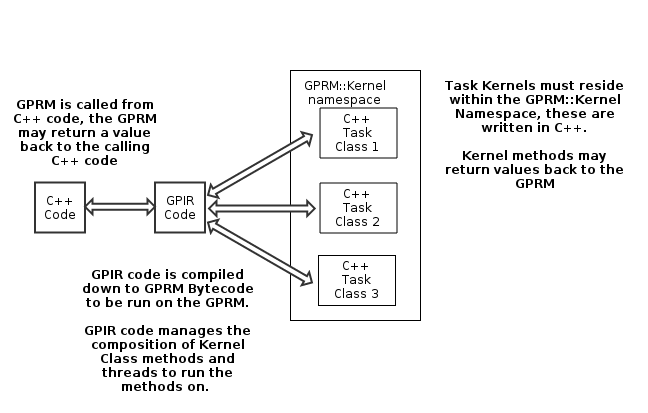
\includegraphics{graphs/gprm.png}
\caption{A simple overview of the GPRM framework}
\end{center}
\end{figure}

\subsection{The GPIR language}

The GPIR language is a purely functional S-expression based language that is evaluated in parallel by default 
with optional sequential evaluation semantics.

Tasks in GPIR are postifxed with a thread number to indicate to the GPRM runtime which thread
the task should run on. For example a simple GPIR program which adds numbers in parallel:

\begin{lstlisting}[style=myGPC]
(begin
    +[0] (+[0] '3 '2) (+[1] '4 '10)
)
\end{lstlisting}

The two nested additions are performed in parallel, with the first being mapped onto thread 0,
and the second being mapped onto thread 1. When they've both been evaluated, then the outer addition
with add the results on thread 0.

\subsubsection{Quoting}

Like in Scheme and Lisp, quoting deffers the evaluation. This is useful for performing sequential evaluation.

\begin{lstlisting}[style=myGPC]
(seq 
    '(obj.m1[0] '1)
    '(obj.m2[0] '2)
)
\end{lstlisting}

Due to the parallel evaluation of GPIR, if the expressions in the seq block wern't quoted then
they would get evaluated in parallel instead of being deffered to be evaluated by the seq function.

Also literal values don't need to be evaluated, they should be deferred and passed to tasks which is
the reason the numbers are quoted in these examples.

The GPIR language has other keywords and features but these are the ones that are important for
understanding the examples and design choices made for this project.

\section{Project Aims}

The GPIR language isn't really suitable for programming in. For one it requires the programmer to manually
manage which thread each task is allocated to. The language is also inconsistant with the C++ language used for 
the other parts of the framework (Calling code and Class Kernels). A language closer to C/C++ will be
more consistent with the entire framework.

The aim of this project is to design a C-like language which can be evaluated in parallel by default, and build
a compiler for it. The compiler should be able to compile this new language down to GPIR code. 

The language should be easy to pick up and write programs in for anyone familiar with the C/C++ languages.
To achieve this the language should be as close to C/C++ as possible 

We'll call the new language being designed " Glasgow Parallel C" or "GPC" for short.

\section{Current C/C++ Parallel Programming Models}

By researching available C/C++ parallel programming frameworks/language extensions 
we can determine possible features and design choices that may suitable for the GPC language.

\subsection{Cilk Plus}

Cilk Plus is a general purpose programming language based on C++. It extends the C++ language with features such as
parallel for loops and spawning functions in parallel using a "fork-join" model to achieve task-parallelism.

One of the main principles of the Cilk language is that abstraction is important and that the programmer should use provided constructs to expose 
the parallelism in their application. This allows the programmer to be free to focus on what the code is allowed to execute in parallel and not worry about the underlying details of manually managing threads. The run-time should then have the responsibility of scheduling the threads and dividing work between
processors.\cite{cilkfaq}. 

Cilk Plus introduces 3 new keywords on top of the C++ language\cite{cilk}: 
\begin{itemize}
    \item \textit{cilk\_for} - Parallelizing for loops, uses the exact same syntax as the standard C++ for-loop
                             with some restrictions.
    \item \textit{cilk\_spawn} - Indicate that a given function can run in parallel with the remainder
                              of the calling function. 
    \item \textit{cilk\_sync} - Wait for all spawned calls to finish.
\end{itemize}

Cilk Plus applications have "serial semantics"\cite{cilk}, this means that the results of an application run
in parallel with Cilk Plus would be exactly the same if it were run
serially (\textit{cilk\_spawn} becoming a function call, removing \textit{cilk\_sync} statements, 
and replacing \textit{cilk\_for} with ordinary for loops).

Cilk Plus makes use of pragmas to indicate to the compiler that a for loop contains data parallelism.\cite{cilkfaq}

Cilk Plus also introduces a new operator \textbf{[:]} to select array sections\cite{cilkarray}. This operator
allows for "high level" operations to be performed on arrays, and can help the compiler vectorize parts of code.

The Cilk Plus runtime makes use of "task stealing" for dynamic load balancing\cite{cilkfaq}. This 
means that if one thread is idle the scheduler can reassign work assigned to be completed by a busier thread. 
The outcome of this is that the programmer doesn't have to worry about the specifics of which threads
to map tasks to, and it can be left to the runtime itself.



\subsection{Open MP}

OpenMP (Open Multi-Processing) is a language extension available for C, C++ and Fortran which allows for shared memory multi-processing. 
This is achieved by the use of compiler directives (more specifically in C/C++ this is done through the preprocessor using pragmas). 
This allows a compiler which doesn't implement OpenMP extensions to still compile C/C++ code
and run it in a linear fashion, and serial code can be made parallel purely through the use of preprocessor
directives without modification to the actual source code.  

\subsection{Intel Thread Building Blocks}

Intell TBB (Intell Thread Building Blocks) is a portable C++ template library for task parallelism.
It contains a range of concurrent algorithms, containers, and it's own task scheduler to achieve this.

Operations are treated as tasks, and the task scheduler has the job of dynamically allocating these tasks 
to individual cores. Abstracting the specific details of allocating threads from the Programmer. 

Using templates allows for 


\section{Wool}
Wool\cite{wool} is a library which is inspired by Cilk that supports task parallel programming by introducing three forms of synchronization. (Create, Exit, and Join). It relies on tasks having low overheads. The 




\chapter{Design}

The goal is to create a C-like language which then compiles down to GPIR code.
The language should be as C-like as possible ideally it should be as much
of a complete subset of C++ as possible.

C++ is a statically typed, imperative language which is sequentially evaluated by default.
GPIR is a dynamically typed functional language which is evaluated in parallel by default.
These two languages use two completely different paradigms, so the language design has to 
ensure that GPC is like C++ and can be compiled to GPIR without too much trouble.

\section{GPC Language Design Decisions}
\label{sec:Lang}

\subsection{Parallel Evaluation}
GPIR is parallel evaluated by default, with a \texttt{seq} function which
evaluates the given arguments in sequential order. Mapping GPC code into
GPIR code which can be evaluated in parallel should be possible, and allows
GPC to take advantage of parallel evaluation by default. GPC should also
have a method of sequentially evaluation of multiple statements.


\subsection{Serial Semantics}
Having serial semantics is helpful to the programmer as it makes
it easy to reason about the behaviour of parallel code.
This is due to the ability to run the entire parallel code in a single
thread as if it were sequential code. 

\subsection{Purely Functional}

In the GPRM jumping to labels is an expensive operation, to avoid
this function calls will need to be inlined, and loops unrolled 
as much as possible. The execution path will also need to be known 
during compile time to achieve this. 

Another one of the major benefits of being able to compute the execution
path at runtime is that recursive functions can be more efficiently parallelized
by the compiler. The following merge sort example is used to illustrate this.

\begin{lstlisting}[style=myGPC]

//Use Sort class from Kernel
GPRM::Kernel::Sort MS;

int size = 8

void merge_sort(int *a, int low, int high) {
    if (low + 1 < high) {
        mid = (low + high) / 2;
   
        seq {
            par {
                merge_sort(a, low, mid);
                merge_sort(a, mid, high);
            }
            MS.merge(a, low, mid, high);            
        }
    
)

void GPC_merge_sort(int *a) {
    merge_sort(a, 0, size);
}

\end{lstlisting}

The merge kernel calls be be reduced down to a tree:

\begin{center}
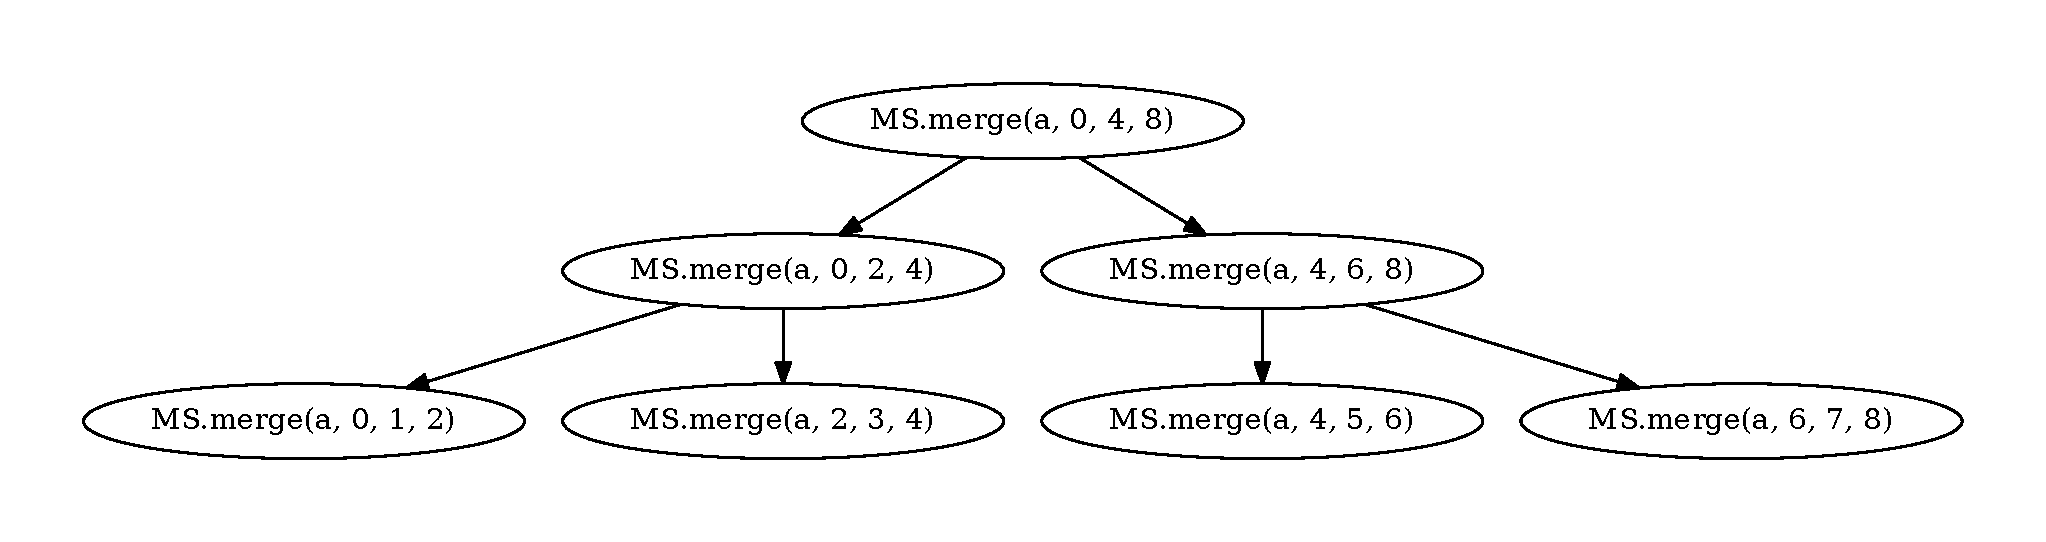
\includegraphics[scale=0.5]{graphs/mergesortTree.pdf}
\end{center}


From the bottom up, the merge operations in the row can be performed in
parallel, knowing the execution path at compile time allows for the compiler
to map these to separate threads. 


However if the language is Turing-complete deciding the execution path
of a given program is essentially the Halting Problem. It has been proven that the solution to this problem is undecidable\cite{halting}. 

To avoid this problem, the language needs to be restricted to a point where it can still be useful and the execution
path decided at compile time.

If the language is purely functional with no side effects then this avoids the problem, however a program
with no side effects is useless. There is one major feature that must ne in the language that invokes
side effects which is method calls for kernel objects. 


To achieve this the type system can enforce that anything returned from a kernel object method call's type then has to be in the 
\texttt{GPRM::Kernel} namespace, and anything passed into a kernel object method call is "cast"into the \texttt{GPRM::Kernel}
namespace. This allows passing impure values between kernel methods but restricts them being used
for conditional statements. Essentially we still have side effects but they're restricted to
only being in Kernel space and not in the GPRM. The execution of GPC code is then purely functional
and the execution path of code can be determined at compile time without too much difficulty.

\section{GPC Language Features}

    This section explains the features of the language with respect to the design decisions in section ~\ref{sec:Lang}.

\subsection{Syntax}
        The syntax aims to be as close to C/C++ as possible. Statements must end with a semicolon. 
        All variables must be statically typed. Blocks are surrounded in braces. Case sensitivity
        will be enforced.

\subsection{New Operators}
        Two new operators not currently present in C++ \texttt{seq} and \texttt{par} are introduced. 
        These are placed before a block
        of statements to determine whether each individual statement within the block are
        to be evaluated in sequential or parallel. By default a block of statements are evaluated
        in parallel, but the par keyword makes it more explicit for readability in the case of lots of nested
        seq/par blocks.

\subsection{Objects}
Objects can be declared in the top level scope, and must be in the GPRM::Kernel namespace.
For example declaring a test object from a class called Test in the \texttt{GPRM Kernel} namespace:

\begin{lstlisting}[style=myGPC]
GPRM::Kernel::Test test;
\end{lstlisting}

Standard C++ method calling syntax can be applied to objects.
\begin{lstlisting}[style=myGPC]
test.m1();
\end{lstlisting}



\subsection{Compatibility with C++}
Making the language completely compatible with C++ in that all GPC code can be
compiled with a C++11 compatible compiler allows programmers that are familiar to
C++ write GPC code with little difficulty. As long as they are aware of the restrictions
that GPC has compared to C++. However the new keywords \texttt{seq} and \texttt{par} are not 
in the C++11 language.

Currently preprocessor directives aren't supported in GPC so the compiler can
just ignore lines starting with \texttt{\#}, and define \texttt{seq} and \texttt{par} as no-ops. 
For example this snippet of code compiles with both the GPC compiler and 
should compile with all C++11 compilers:

\begin{lstlisting}[style=myGPC]
#include "GPRM/Kernel/Test.h"
#define seq
#define par

GPRM::Kernel::Test test;

int entry_fn() {
    seq {
        int a = test.m1();
        int b = test.m2(a);        
        par {
            test.m3(b);
            test.m3(b + 1);
        }
        return 0;
    }
}
\end{lstlisting}

When this code is compiled with a C++ compiler it will removed the seq and par
keywords and what will be left is plain blocks. Essentially this should generate a
serial version of the program which should generate the exact same results
as the version compiled by GPC and run on the GPRM. This supports the 
design decision of serial semantics.

This is useful for implementing the compiler as it allows for
testing that the code generated by GPC is generating the correct results
by comparing it to the C++ version. It also allows for easier porting of
programs already written in C++ to GPC. Programmers can use tools
already made for C++ to debug their serial code before attempting
to run it in parallel on the GPRM.

However this method restricts the possible implementation of pragmas
into the GPC language in the future. A possible improvement would be to change
from the cilk plus approach of adding extra keywords to the language to an openMP
approach of having \texttt{seq} and \texttt{par} pragmas instead. Then the language
would be fully compatible with C++ without needing to modify the GPC code.

\subsection{The Type System and Kernel restrictions}
        C++ types such as string, char, bool, int, and double are included.
        Pointers, and "multilevel" pointer types are included (e.g. int**, char*).
        However pointers are restricted in that the address of a variable
        cannot be taken. Adding and subtracting integers
        from pointers is allowed. Usually pointers are passed into
        the GPRM from the C++ caller to represent an Array.

        Return values from kernel method calls are implicitly placed
        in the \texttt{GPRM::Kernel} namespace. 

For example:

\begin{lstlisting}[style=myGPC]
int x = obj.method(5);
\end{lstlisting}

This is implicitly cast to:

\begin{lstlisting}[style=myGPC]
GPRM::Kernel::int x = obj.method(5);
\end{lstlisting}     

If a binary expression involved a Kernel value and a "pure" value
then the "pure" value is implicitly upcast before the operation takes
place. For example:

\begin{lstlisting}[style=myGPC]
bool y = obj.m1(10) == 5;    
\end{lstlisting}

is implicitly cast to:

\begin{lstlisting}[style=myGPC]
GPRM::Kernel::bool y = ob.m1(10) == 5;
\end{lstlisting}

This feature stops impurity in the GPC code execution, as the type system
should be able to stop Kernel types being used in conditional
statements. 

For example this is not allowed:
\begin{lstlisting}[style=myGPC]

seq {
    int x = obj.method(5);
    if (x == 10) {
        //Do Stuff
    }    
}

\end{lstlisting}

If statements must take a "pure" boolean type as its conditional.
\texttt{x == 10} is a \texttt{GPRM::Kernel::bool} type, so this raises a type error.
  
\subsection{Operations}
        Most basic binary arithmetic operations are included i.e. 
        (+, -, *, /, \%, ==, !=, \&\&, $||$ , \lstinline|<<|, \lstinline|>>|, \lstinline|&|, $|$, 
        \lstinline|^|) as well as
        unary operations 
        (\lstinline|-|, \lstinline|~|, \lstinline|!|).

        (+=, ++, --, -=) are not included, due to the single assignment rule.
        Although an exception is made for the "afterthought" of the for loop construct, in which
        the integer loop variable can be incremented with += or decremented by -=.

\subsection{Functions}
 Basic support for defining and calling functions is supported, and function  
 syntax is exactly the same as C. However there is currently no
 support for function pointers and C++11 lambdas. 


\subsection{Single assignment}
Variables in GPC can only be assigned once per scope to keep
the language functional.

for example the following isn't allowed:

\begin{lstlisting}[style=myGPC]
int i = 0;
int i = i + 1;
\end{lstlisting}

Since \texttt{i} is already in scope, it cannot be redefined in the same scope.

The following code is allowed:

\begin{lstlisting}[style=myGPC]
int i = 0;
{
   int i = i;
}
\end{lstlisting}

Since \texttt{i} inside the block is declared in a new scope.

Also variables must be assigned when they are declared, for example the following is not allowed:

\begin{lstlisting}[style=myGPC]
int x;
x = 5;
\end{lstlisting}

\subsection{For-Loops}
For loops have the same syntax as C/C++ for loops with some restrictions:

\begin{itemize}
\item There is a single loop variable which must be declared inside the loop, and must be an integer.

\item The conditional expression must result in a "pure" boolean type, a \textit{GPRM::Kernel::bool}
     type is not allowed.

\item The "afterthought" of the for loop must consist of the loop variable with either the \texttt{+=} operator
      or \texttt{-=} operator with a "pure" integer value on the right hand side. This is the only place these
      binary operations are allowed to occur in a GPC program. 

\end{itemize}

These restrictions and properties are in place to keep the functional "purity" of GPC code,
allowing complete compatibility with the C++ language, and keeps the property of GPC programs
having serial semantics.  
At compile time the loop is fully unrolled, these restrictions also allow for detection
at compile time whether or not the loop is infinite.  

It's worth noting that these restrictions are similar to the restrictions on the \textit{cilk\_for} loop.
The \textit{cilk\_for} loop must declare a single initial loop variable, the conditional expression must 
compare the loop variable with a constant "termination expression", and the "afterthought" must either increment
or decrement the loop variable by some amount
\cite{cilkfor}.

An example of a for loop is as follows:


\begin{lstlisting}[style=myGPC]
for(int i = 0; i < 5; i+=1) {
    obj.m1(i);
}
\end{lstlisting}


During compilation this loop is fully unrolled and is equivalent
to the following:

\begin{lstlisting}[style=myGPC]
par {
    obj.m1(0);
    obj.m1(1);
    obj.m1(2);
    obj.m1(3);
    obj.m1(4);
}
\end{lstlisting}


\subsection{Top Level Statement Restrictions}
Top Level statements are restricted to being either object declarations, function definitions,
or constant variable assignments. This is partly to be like C++ and also to remove any ambiguity
on how top level statements are evaluated.


\subsection{Entry Function}
Since the GPIR function is called by C++ code, it's not preferable to name the function "main".
Also the C++ code may be calling more than one GPIR function during its lifetime so a static
name is also not preferable. The GPIR code entry function has the same name as the GPC source
file it is in. For example the entry function  for "test.gpc" would be called "test". This method
of determining an entry function is not ideal, but is easy to change in the future if needed.






\chapter{Implementation}


\section{Implementation Language Choice}

The compiler will be implemented using the Haskell programming language.

During complication the need to traverse trees usually occurs quite
often. Functional languages like Haskellare suited to this task 
due to features such as pattern matching and tail-end recursive optimisation 
which make traversing trees efficient and simple to implement/ 

The Glasgow Haskell Compiler is available for most platforms, most importantly for Windows, OSX and Linux 
on x86 architectures. This allows the compiler to be portable across these platforms provided the libraries 
used to build the compiler are portable.

Haskell has algebaric datatypes, these makes Abstract Syntax Trees
simpler to implement. For example the AST for a very simple expression
can be representedas follows:

\begin{lstlisting}[style=myHaskell]

    data Expression =
          Add Expression Expression
        | Negate Expression 
        | Const Integer

\end{lstlisting}

The equivalent in an Imperative/OOP language (in this case Java)
would be the following:

\begin{lstlisting}[style=myJava]

abstract Class Expression {}

class Add extends Expression {
    public Expression left;
    public Expression right;
    public Add(Expression l, Expression r) {
        left = l;
        right = r;    
    } 
}

class Negate extends Expression {
    public Expression expr;
    public Negate(Expression e) {
        expr = e;    
    }
} 

class Const extends Expression {
    public int value;
    public Const(int v) {
        value = v;
    }
}       

\end{lstlisting}

The Haskell version is much clearer on the structure of the tree, and takes much
less code to implement. 

It is also to easily extend Haskell datatypes to include
custom annotations. For example storing the source code position for parts of expressions may
be useful for reporting errors to the user.

Due to the pure function nature of Haskell, parts of complilation can easily be performed in parallel.
For example during type checking, each GPC function can be type checked in parallel and this can even be subdivided 
further into blocks within functions. For this project speed of compilation is not a major concern, but in the future if compliation ever
needs to be faster then this option is always available.

Haskell also has powerful libraries for parsing source code such as Parsec which is a parser combinator
library. Parsec allows Combinator parsers to be written in the Haskell language itself avoiding the complexity
of integration of different tools and languages\cite{parsec}. 

\section{Tools and Testing}


\subsection{Cabal}

Cabal (Common Architecture for Building Applications and Libraries) is a system for building and
packaging Haskell libraries and programs.\cite{cabal}. This system can manage the
project library dependencies, and automatically download and install missing dependencies.
It can also build amd install the compiler on the system, and run unit tests.

\subsection{Testing}

For Unit testing the HUnit library will be used, this can be integrated
with Cabal to easily run all the required unit tests.

One form of testing used for this project is testing each individual component
(e.g. The Parser or the TypeChecker). Each component in the compiler can easily
be uncoupled from one another due to the linear nature of compliation.

Another form of testing is writing GPC source files which should compile, and
GPC files which should fail compilation at a certain stage. The compiler
is then invoked during testing on all of these files to check whether
all the source files which should compile do infact compile with no errors,
and all the source files which should raise an error do not compile.

An upside to this method is that testing this way is flexible in that
they aren't coupled with the implementation internals of the compiler.
The only way that these test would need to be changed was if the design
of the language itself would need to be changed.

The downsides to this method is that without manually checking the errors raised
by the tests that should fail the source may generate an error which is unrelated
to the error that is being tested. This is why some testing of each internal
component is done alongside this method.

\subsection{Code Coverage}

The Haskell HPC (Haskell Program Coverage) library allows for recording
code coverage over different modules during testing. This can be integrated with
cabal unit testing to automatically generate these results. The usefulness of this
allows for checking which sections of code still need to be tested and assists
in writing further unit tests.


\section{Compiler Structure}
Compilation is split up into multiple stages or "passes",
it is possible to compile in one pass but seperating each 
specific section of compilation allows modularity and decoupling.

\newpage
\begin{figure}[!htb]
\begin{center}
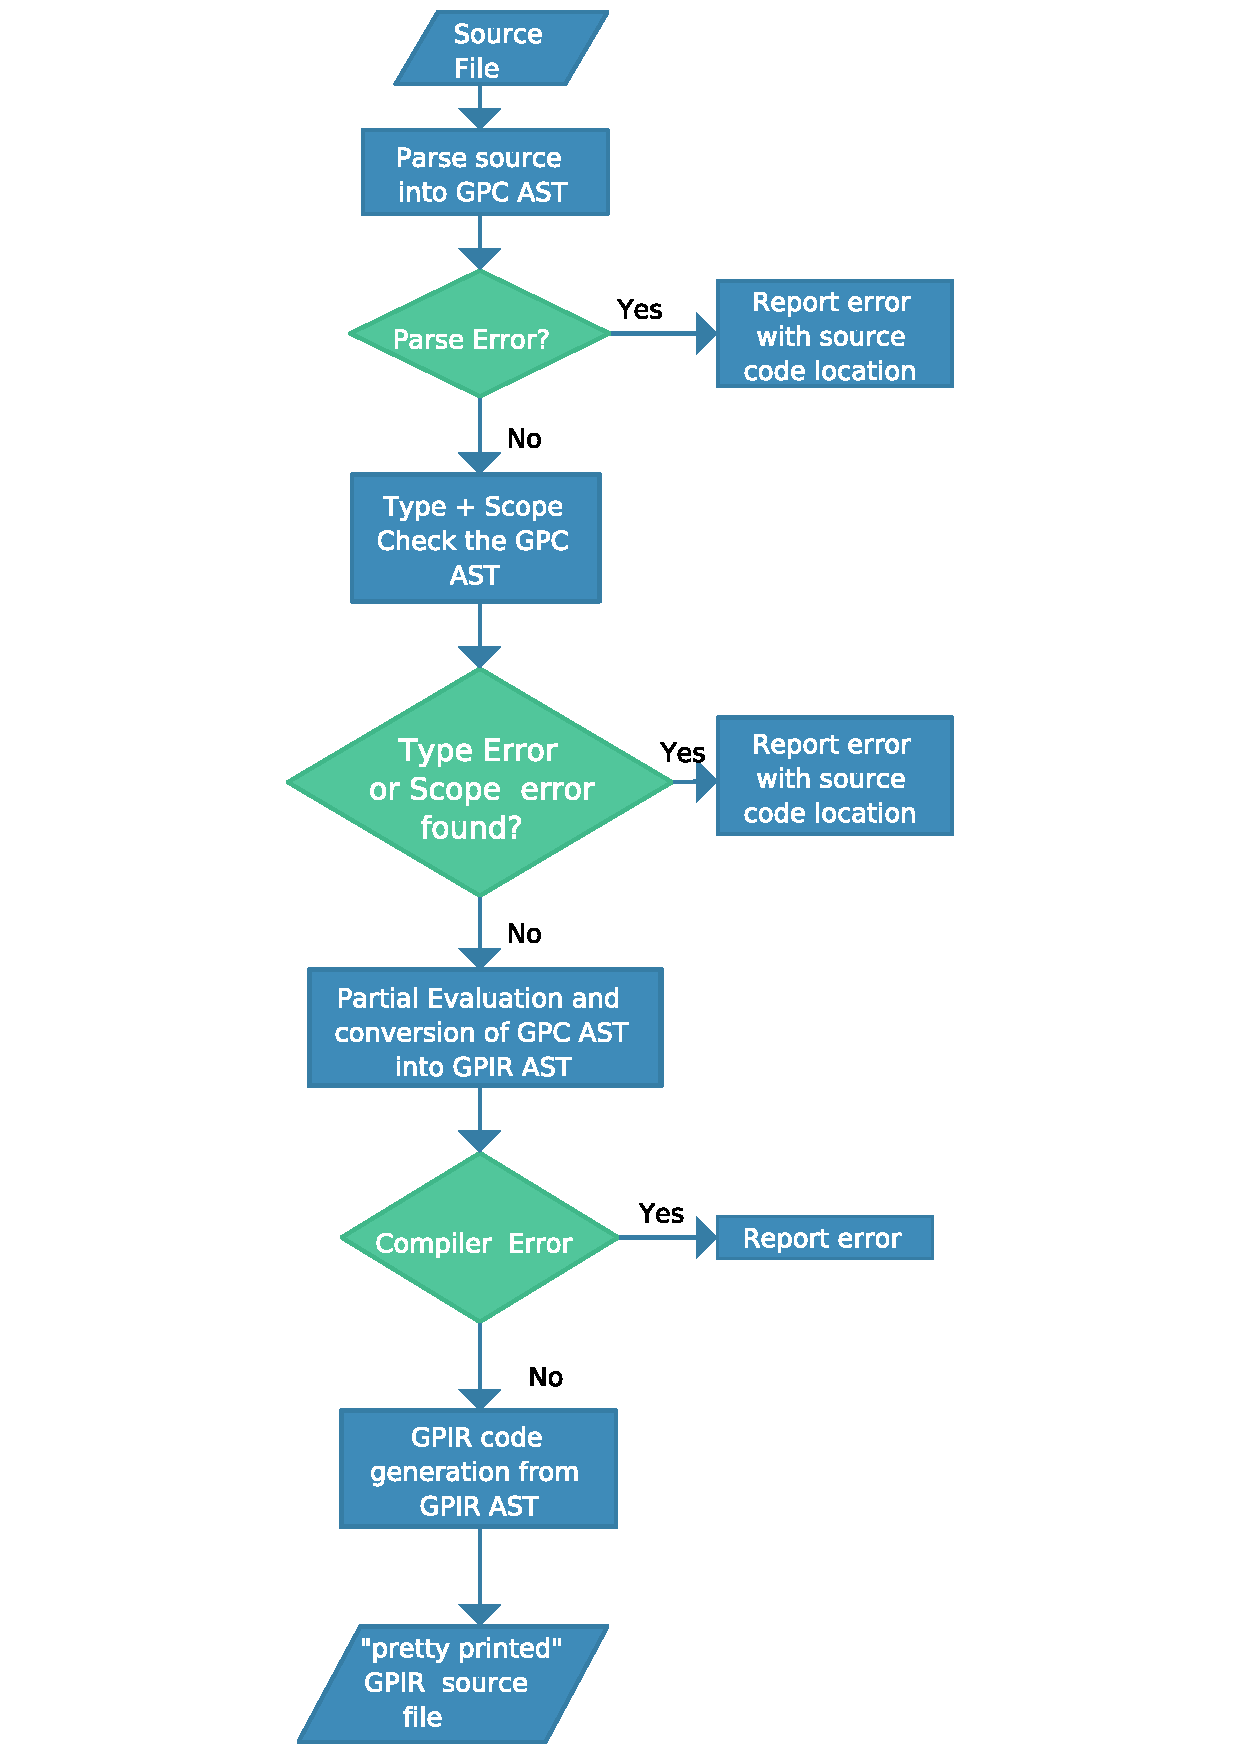
\includegraphics{graphs/Dissertation.pdf}
\caption{Flowchart illustrating the stages of the GPC compiler.}
\end{center}
\end{figure}

    
\subsection{Parser/Lexer}
The Parsec library combines Parsing and Lexing into one stage.

Given the GPC source file the intention is to parse the file into an AST
to hopefully eventually be transformed into GPIR source code. It's
also useful to store the original source position to provide error information 
during a further compilation stage, to achieve this the source position
info is read from Parsec into an Annotated AST as the tree is being built up.

Parsec does most of the work during this stage, including
providing error messages for "expected" values to be found in source
positions and source position information. Most of the work implementing
this stage is building the parser combinator functions and composing
them together to be able to build the AST.


\subsection{Type and Scope checking}

During type checking the types of identifiers from the current scope being used in expressions need
to be known. Since the scope needs to be kept track of while type checking it makes reasonable
sense to check for scope errors in the same stage.

The goal of this stage is to ensure that the static typing of the source file
is enforced (e.g. attempting to assign a bool value to a variable of type int should not happen) and,
prevent "logic" errors at compile time (e.g. adding 2 bool values together). Scope checking
is also important as identifiers being used within the program need to be binded to an expression of
some sort, and the "single assignment" rule in the GPC language needs to be enforced.

There are two seperate "types" of scope in a GPC program. The first is the top level scope and the
other is at function level scope. Any scope "further" down from function level scope is itself
a function level scope. During this stage the top level scope will be type and scope checked.
Afterwards each individual function will be type and scope checked.

For checking over top level statements the following Haskell record is used
to keep track of identifier types, objects, and functions encountered:

\begin{lstlisting}[style=myHaskell]
type VarTable = M.Map (Ident SrcPos) (Type SrcPos)
type FunTable = M.Map (Ident SrcPos) (Type SrcPos, [Type SrcPos])
type ObjectTable = M.Map (Ident SrcPos) (Objects SrcPos)

data MainBlock = MainBlock {
    _tlFuncDefs      :: FunTable, -- ^ Function Definitions
    _tlVarTypes      :: VarTable,  -- ^ Top Level Constant variable types
    _objects         :: ObjectTable  -- ^ Table of current Kernel objects declared 
} deriving (Show)
\end{lstlisting}

It needs to be checked that no duplicate functions exist and  no duplicate top level variables exist,
Once all top level statements have been checked, all functions in scope stored, 
all top level variables stored, and all variables stored. Each individual function
can be checked.

A slightly different stucture is needed to type check functions.

At anytime it is needed to be known what variables that are currently in scope, their types,
what functions are avilable to call, their argument types, and return types. Also the
objects which are available to call methods on, and the current function the type checker
is in at any point.

These values can be stored using the following Haskell record: 

\begin{lstlisting}[style=myHaskell]

data CodeBlock = CodeBlock {
    _currentFun :: Ident SrcPos, -- ^ Name of Function block is in
    _funcDefs   :: FunTable, -- ^ Function names and return/argument types
    _prevVars   :: VarTable, -- ^ Identifiers visible in current scope with types
    _curVars    :: VarTable  -- ^ Identifiers declared in current scope
} deriving (Show)


\end{lstlisting}

When a function is being type check a new CodeBlock instance needs to be
created from a MainBlock instance, as some of the top level information is needed.
The details of the function that is being entered is stored in "\_currentFun", 
details of all available functions stored in "\_funcDefs", and store all
top level variable in "\_prevVars". "\_curVars" is left as an empty map as the
type checking of the function hasn't begun yet. Top level objects are also
stored in "\_curVars" as an "object" variable type.

Whenever a new scope is encountered by either calling a function, or entering a seq/par block;
A new CodeBlock structure is created using the current structure. The new "\_curVars"
is set to the empty map as no variables have been encountered yet, the "\_funcDefs"
are copied as all functions are on the top level so they don't change. The "\_currentFun"
is copied if entering a block, otherwise if entering a function the function name
and source position are copied. 

The value of the new "\_prevVars" is a little more complicated to work out.
Any key, value pairs in the current "\_curVars" are stored plus any key, value
pairs in the current "\_prevVars" in which the key isn't present in the current 
set of "\_curVars" keys. This is because
the identifiers in "\_curVars" scope are visible over the identifiers with
the same name in "\_prevScope". Haskell's union operation on maps
discards the key, value pairs in the second map for keys that are
present in the first map, so this is trivial to implement.

When type checking a function, every statement in the function is type checked
as well as the type of the return statement. For every statement,
every expression within the statement is type checked. This is implemented by traversing
the Statement AST and checking the scopes of identifiers as well as expected types
against actual types.

Objects which are declared are not checked to see if they actually exist. Neither
are method calls which means the argument types and return types when calling them
cannot be determined at compile time. This is due to the fact Objects are written
in C++, and the C++ class would need to be checked for methods and types. This is already
implemented in the GPRM, so an error will occur further down to compile "chain" or during
runtime.

If a type or scope error is encountered, an error message determining the type of error,
and the source position of the error is returned. Otherwise an empty tuple is returned.
When type and scope checking the original AST doesn't need to be modified, only verified
that it follows the type and scope rules of the language.


\subsection{Evaluation}

The goal of this stage is to run through the execution path the GPIR code
will take from the entry function, and partially evaluate the code as much
as possible while generating the GPIR AST.

Just before Evaluation the AST is transformed slightly into a similar AST
with two differences. One is that annotations are not present (since source position information
is not needed anymore), and type information is stripped (since the program has been proven to 
not have any type errors).




\begin{lstlisting}[style=myHaskell]

type ConstVarTable = M.Map Ident Literal
type FunTable = M.Map Ident ([Ident], BlockStmt)
type VarRegTable = M.Map Ident Integer

-- ^ Current State of the Block we are currently in
data CodeGen = CodeGen {
   _funTable    :: FunTable,  -- ^ Store symbol tree for functions
   _constTable  :: ConstVarTable, -- ^ Store constants in scope
   _varId       :: Integer, -- ^ Current variable id for mapping to registers
   _varRegTable :: VarRegTable, -- ^ maps variable identifier
   _threadCount :: Integer, -- ^ Current thread number to map
   _maxThreads  :: Integer,  -- ^ Maximum number of threads
   _seqBlock    :: Bool, -- ^ Whether or not current block is sequential
   _isReturning :: Bool -- ^ Whether the state of the current block is in a return
}

\end{lstlisting}

\subsection{GPIR Code Generation}






\chapter{Future Work}

Future Features that could be added:

\section{Configuration file generation}
    yml config generation.
    These files are needed by the GPRM to determine aliases in GPIR code, libraries used,
    number of threads/nodes. There is enough information at compilation time to generate these,
    and they are currently generated manually. 


\section{Language Features}
    Other C++ language features, C++11 lambdas may be useful,
    while-loops, and possibly some STL support e.g. ability to use STD vector instead of pointers.

\section{Compiler Optimisations}

    There are a few optimisations that can be performed by the compiler to reduce the work needed to be 
    performed by the GPRM at runtime.

\subsection{Binary Expression Reduction}
Given the following GPC code:    

\lstinputlisting[style=myGPC]{code_samples/binaryOp.gpc}

In line 8, the expression within the m2 method call results in part of the Abstract Syntax Tree
which is represented as a Binary Expression Tree when parsed. Binary operators are contained in
the inner nodes with literal values and variables at the leaf nodes. 

\begin{center}
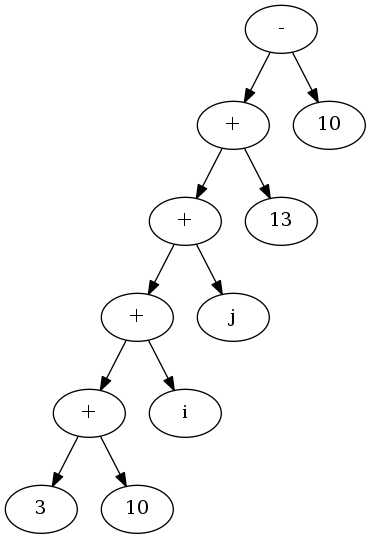
\includegraphics[scale=0.4]{graphs/evalTree.png}
\end{center}

During the evaluation stage of compilation the tree is evaluated through
postorder traversal. Once two leaf nodes are found the binary operation in the parent node
is attempted to be applied to the two leaf nodes. If both leaf nodes are values which
can be calculated at compile time the expression is evaluated, the two leaf nodes
are removed and the parent node is replaced with the calculated value. If one or
more leaf nodes are values which can only be known at runtime then the expression is
not evaluated and the tree doesn't change. 

The tree above once evaluated transforms into the following tree: 

\begin{center}
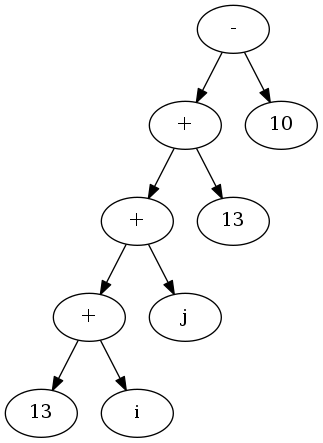
\includegraphics[scale=0.4]{graphs/fullyEvalTree.png}
\end{center}

We can see this reduction in the generated GPIR code:

\lstinputlisting[style=myGPIR]{code_samples/binaryOp.td}

The downsides of this method is that once
a value that can't be worked out at compile time is met, it is not possible
to evaluate expressions any value further up the tree. In the given example
it is clear that it is possible to evaluate the expression further.

One way to improve the evaluator would be to transform the tree before evaluating it.
Using the axioms of the binary operations in the tree (e.g. addition being associative)
and the type of values in the leaf nodes,. it should be possible to rearrange the nodes in the 
tree to create a new tree which represents an expression equivalent to the expression
represented by the starting tree.

The specific details of how the tree transformations work and implementation into the compiler is 
left as future work.

In this example, one "optimal" transformation of the tree would result in the following tree:

\begin{center}
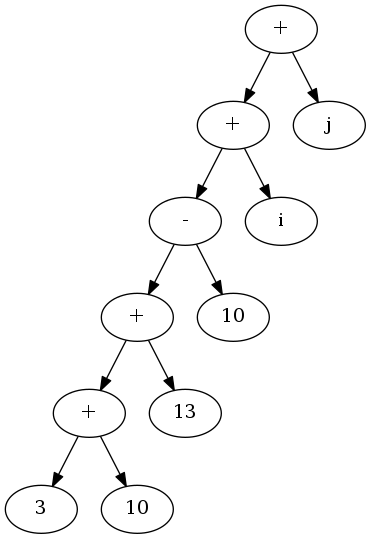
\includegraphics[scale=0.4]{graphs/optimalEvalTree.png}
\end{center}

The evaluator would then reduce this tree down to the following tree:

\begin{center}
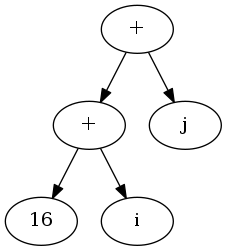
\includegraphics[scale=0.4]{graphs/optimalFullyEvalTree.png}
\end{center}

This generates much simpiler GPIR code:
\lstinputlisting[style=myGPIR]{code_samples/binaryOpImproved.td} 


\subsection{Pure Function Reduction}

When a function is pure (i.e. it contains no method calls
on kernel objects, and all arguments given to it when it is called can be evaluated at 
compile time) the function call should be able to be evaluated down to a single constant value.

The following GPC code is used as an example:

\lstinputlisting[style=myGPC]{code_samples/pureFun.gpc}

The function "f" does not call any methods on kernel objects, and has no arguments.
Every time "f" is called it returns the integer value "2". Therefore wherever f is called can
be replaced with the integer value "2". However the compiler generates the following GPIR code
for this example:

\lstinputlisting[style=myGPIR]{code_samples/pureFun.td}

When "f" is called its value is stored in a register. This is currently how function calls
store their return value when evaluated. An improvement to function evaluation to support
reduction of "pure functions" would result in generating this simpler GPIR code:

\lstinputlisting[style=myGPIR]{code_samples/pureFunImproved.td}




%%%%%%%%%%%%%%%%
%              %
%  APPENDICES  %
%              %
%%%%%%%%%%%%%%%%
\begin{appendices}
\end{appendices}

%%%%%%%%%%%%%%%%%%%%
%   BIBLIOGRAPHY   %
%%%%%%%%%%%%%%%%%%%%

\bibliographystyle{plain}
\bibliography{bib}

\end{document}
